\chapter{Il processo di certificazione e di accreditamento}
\section{Introduzione}
Questo capitolo affronterà la certificazione di sicurezza in ambito di \textit{web-services}, illustrando i criteri, le metodologie e i paradigmi implicati.
Per "\textit{certificazione}" si intende l'insieme di procedure impiegate nel processo di erogazione di un certificato, ovvero la produzione di un documento attestante la compatibilità tra le caratteristiche di un sistema o di una procedura e i requisiti prestabiliti da una norma o da uno standard.
L'"\textit{accreditamento}" è invece la dichiarazione formale da parte di una terza parte fidata che il processo di certificazione sia a sua volta compatibile con uno standard riconosciuto.
In ambito di sicurezza informatica, certificazione e accreditamento possono essere intesi come parti di un unico processo: \textit{Certification and Accreditation (C\&A)} \cite{NistCAHandbook}.

La fase di certificazione comprende un'analisi del sistema per identificare le possibili debolezze e le relative contromisure in un particolare ambiente e un'analisi delle potenziali vulnerabilità causate dalle debolezze individuate \cite{NistCAHandbook}.
La fase di accreditamento rappresenta invece la dichiarazione formale da parte di una "autorità designata all'approvazione" (\textit{Designated Approving Authority, DAA}) che un sistema informatico  automatizzato \textit{(Automated Information System, AIS)} operi in una determinata modalità di sicurezza utilizzando un insieme predefinito di protezioni basato sul rischio residuo identificato durante il processo di certificazione \cite{NistCAHandbook}.

L'accreditatore ha quindi la responsabilità formale di autorizzare l'operatività del sistema e deve rimanere impegnato attivamente nel processo di riaccreditazione durante il ciclo di vita di un sistema, poiché il livello di rischio può cambiare \cite{NistCAHandbook}.
Il processo di accreditazione deve essere implementato all'inizio del ciclo di vita del sistema, per garantire
\begin{itemize}
\item che siano progettati e integrati i meccanismi di sicurezza e le protezioni opportune
\item che le decisioni di sicurezza non vengano ritardate causando costi aggiuntivi
\end{itemize}


\section{Valutazione del software sicuro basata sui \textit{Common Criteria}}
Tradizionalmente, le tecniche di certificazione rappresentano la soluzione di analisi scelta per fornire la prova che un software abbia le proprietà non funzionali desiderate e si comporti come atteso.
Sono state proposte molte soluzione e schemi, alcuni di essi si sono concentrati sulla certificazione delle proprietà di sicurezza del software.\cite{CitCertSoa}
Il primo tentativo in questa direzione risale al 1985, con la creazione dello standard TCSEC, comunemente chiamato "\textit{Orange Book}"\cite{OrangeBook}.
Successivamente sono stati proposti altri standard, come il Common Criteria del Dicembre 1999, (ISO15408) che rappresenta il punto di riferimento internazionale per la certificazione del software sicuro.\cite{HerrmannCC}






\section{Certificazione dei servizi SOA basata sul testing}
%integrare Security Certification of Composite Services: A Test-Based Approach
Le tecniche di certificazione possono giocare un ruolo molto importante anche nell'ecosistema dei servizi, tuttavia le modalità esistenti non si adattano bene a questo scenario. Un ecosistema basato sui servizi è, per definizione, di natura dinamica; le tecniche di certificazione usuali, invece, considerano il software come entità statica e monolitica, fornendo un certificato non formalizzato e utilizzabile solo nella fase di installazione del prodotto.
Abbiamo dunque bisogno di una soluzione che possa essere integrabile nella composizione dei processi di business.\cite{DamianiCitCertSoa} 
\cite{CitCertSoa}

Un approccio potenzialmente in grado di garantire le esigenze di certificazione per i servizi web, è stato definito nell'articolo \textit{A Test-Based Security Certification Scheme for Web Services} di \textit{Anisetti, M. , Ardagna, C. , Damiani E. e Saonara F.}\cite{CitCertSoa} e si basa su un modello fondato sul testing per fornire le prove che il servizio da certificare rispetti un insieme di proprietà di sicurezza date.
Lo schema di certificazione si basa su casi di test generati automaticamente, in modo da produrre evidenze \textit{machine-readable} per comprovare le proprietà di sicurezza del servizio.\cite{CitCertSoa}

\subsection{Processo di certificazione}


L'obiettivo della certificazione è rappresentato dalla proprietà di sicurezza da certificare.
Il processo descritto è fondato sulla certificazione delle proprietà di sicurezza (confidenzialità, integrità, autenticità), e ha inizio da un \textit{service model} che contiene tutte le informazioni di interesse per effettuare il processo di certificazione.
A partire da esso si producono le evidenze a sostegno della proprietà da certificare.
Alla conclusione del processo, si può affermare che una data proprietà di sicurezza è certificata in base a un determinato \textit{service-model} (Figura \ref{fig:CertSoaFig1a}).

\begin{figure}[H]
\centering
\makebox[\textwidth]{
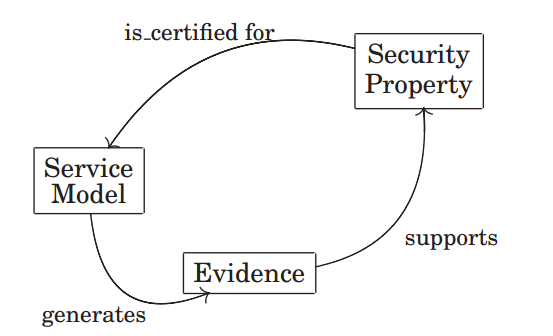
\includegraphics[width=8cm]{immagini/CertSoaFig1a.png}
}
\caption{Fasi del processo di certificazione\cite{CitCertSoa}}\label{fig:CertSoaFig1a}
\end{figure}

Il processo  e viene condotto grazie alla collaborazione di tre attori, la cui interazione è descritta nella figura \ref{fig:CertSoaFig1b}:
\begin{enumerate}
\item Un fornitore di servizi, che necessita della certificazione. Implementa il proprio servizio web e produce:
\begin{itemize}
\item il documento di descrizione delle operazioni in "\textit{Web Service Description Language (WSDL)}".
\item il documento di descrizione delle interfacce e di conversazione con i client in "\textit{Web Service Communication Language (WSCL)}".
\end{itemize}
Dopodiché avvia il processo di certificazione, fornendo all'autorità di certificazione i documenti WSDL e WSCL, l'implementazione del servizio e la lista delle proprietà da certificare. 
\item Un'autorità di certificazione (\textit{certification authority}) che gestisce tutto il processo di certificazione. Una volta ricevute le informazioni dal fornitore di servizi, genera il \textit{service model} e lo invia a un laboratorio accreditato insieme all'implementazione del servizio, e alla lista delle proprietà di certificare, fornite al punto 1.
\item Un laboratorio accreditato (\textit{accredited lab}) controllato dall'autorità di certificazione, che  effettua la valutazione delle proprietà. Una volta ricevute le informazioni dalla \textit{certification authority}, effettua la fase di generazione delle evidenze e le restituisce alla stessa. Se queste sono sufficienti, la \textit{certification authority} rilascia un certificato per il servizio, includendo proprietà certificate, il \textit{service model} e le evidenze.
\end{enumerate}

\begin{figure}[H]
\centering
\makebox[\textwidth]{
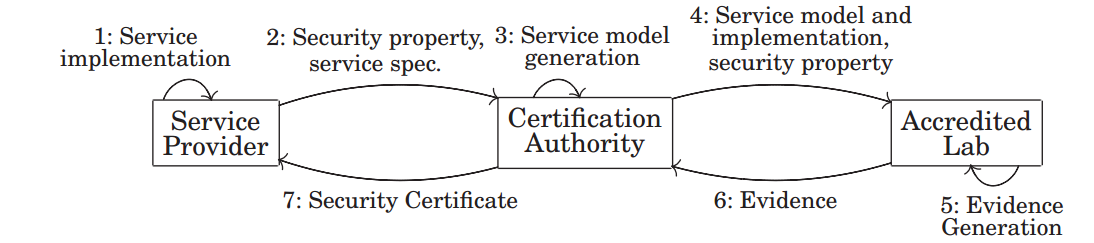
\includegraphics[width=\textwidth]{immagini/CertSoaFig1b.png}
}
\caption{Fasi del processo di certificazione\cite{CitCertSoa}}\label{fig:CertSoaFig1b}
\end{figure}

\section{Certificazione incrementale} %A Low-Cost Security Certification Scheme for Evolving Services
